%!TEX root = ../main.tex

\section{\texorpdfstring{$\CP$}{CP} violation in \texorpdfstring{$\bToccbars$}{bToccbars} decays (2 pages)}
\label{sec:cpviolation:btoccbars}

The gold-plated mode to measure \CP violation in the system of neutral $B$
mesons is \BdToJPsiKS. It proceeds via a \bToccbars transition. Direct and
indirect \CP violation is strongly suppressed, which makes it a very clean
mode to determine the weak mixing phase, and thus the CKM angle $\beta$, via
\CP violation in the interference of decay and decay after mixing. As the
Feynman diagrams in \cref{fig:cpviolation:bd2jpsiks_feynmans} show, actually
\BdToJPsiKz and \BdbToJPsiKzb decays take place.
\begin{figure}[htb]
\centering
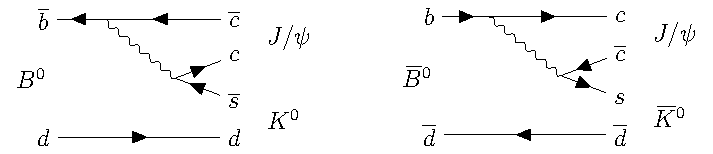
\includegraphics[width=\textwidth]{03-CPViolation/tikz/pdf/BdToJPsiKS.pdf}
\caption{Tree Feynman diagrams of \BdToJPsiKS for both flavours.}
\label{fig:cpviolation:bd2jpsiks_feynmans}
\end{figure}
However, like for the $B$ mesons the flavour eigenstates are a superposition
of the \CP mass eigenstates:
\begin{align}
	\ket{\KS} = p_K \ket{\Kz} - q_K \ket{\Kzb}
\end{align}
Therefore, the ratio of decay amplitudes is composed of two terms according to
\begin{align}
	\frac{\bar{A}_{\JPsi\KS}}{A_{\JPsi\KS}} = -\frac{p_K}{q_K}\frac{\bar{A}_{\JPsi\Kzb}}{A_{\JPsi\Kz}}\,.
\end{align}
The ratio of the mixing coefficients for the kaons can be calculated using
\cref{eq:cpviolation:qp}. Different than for the $B$ mesons the dominant
contribution to the mixing diagrams arises from charm quarks in the loop:
\begin{align}
	\frac{p_K}{q_K} = -\frac{\Vcs\Vcds}{\Vcss\Vcd}
\end{align}
Accounting only for the tree diagrams in
\cref{fig:cpviolation:bd2jpsiks_feynmans}, while neglecting loop processes,
the ratio of the direct decay amplitudes can be expressed via the involved CKM
matrix elements:
\begin{align}
	\frac{\bar{A}_{\JPsi\Kzb}}{A_{\JPsi\Kz}} = \frac{\Vcb\Vcss}{\Vcbs\Vcs}
\end{align}
Summarising these values and adding the ratio of CKM matrix elements for the
mixing of the \Bd mesons (see \cref{eq:cpviolation:qp_simplified}) the
parameter describing \CP violation from \cref{eq:cpviolation:lambda} becomes
\begin{align}
	\lambda_{\JPsi\KS} = - \frac{\Vtbs\Vtd}{\Vtb\Vtds}\frac{\Vcs\Vcds}{\Vcss\Vcd}\frac{\Vcb\Vcss}{\Vcbs\Vcs} = - \frac{\Vtbs\Vtd}{\Vtb\Vtds}\frac{\Vcds\Vcb}{\Vcd\Vcbs}
\end{align}
The minus sign indicates that the final state $\JPsi\KS$ is \CP-odd, as an
angular momentum of $l = 1$ is necessary to compensate that the \Bd meson as
initial state has spin zero, while the final state consists of a \CP-even
$\JPsi$ meson with spin one and an almost \CP-even\footnote{When reconstructed
in a pair of two pions it is fully \CP-even.} \KS meson with spin zero.